
%(BEGIN_QUESTION)
% Copyright 2010, Tony R. Kuphaldt, released under the Creative Commons Attribution License (v 1.0)
% This means you may do almost anything with this work of mine, so long as you give me proper credit

Determine the effect(s) of each fault -- considered one at a time -- on the operation of this nondispersive infrared (NDIR) analyzer:

$$\includegraphics[width=15.5cm]{i00758x01.eps}$$

\begin{itemize}
\item{} Chopper wheel stops spinning
\vskip 10pt
\item{} Leak develops in chamber 2
\vskip 10pt
\item{} Leak develops in chamber 4
\vskip 10pt
\item{} Parabolic mirror cracks
\end{itemize}

\underbar{file i00758}
%(END_QUESTION)





%(BEGIN_ANSWER)

\begin{itemize}
\item{} Chopper wheel stops spinning: {\it the analyzer's output will go to zero for all gas concentrations.}
\vskip 10pt
\item{} Leak develops in chamber 2: {\it a ``zero'' shift will develop.}
\vskip 10pt
\item{} Leak develops in chamber 4: {\it there may be no effect, unless the ambient air carries a significant concentration of interferent gas.}
\vskip 10pt
\item{} Parabolic mirror cracks: {\it zero shift, depending on the location and severity of the crack.}
\end{itemize}


%(END_ANSWER)





%(BEGIN_NOTES)


%INDEX% Measurement, analytical: nondispersive optical

%(END_NOTES)

